%%%%%%%%%%%%%%%%%%%%%%%%%%%%%%%%%%%%%%%%%
% Beamer Presentation
% LaTeX Template
% Version 1.0 (10/11/12)
%
% This template has been downloaded from:
% http://www.LaTeXTemplates.com
%
% License:
% CC BY-NC-SA 3.0 (http://creativecommons.org/licenses/by-nc-sa/3.0/)
%
%%%%%%%%%%%%%%%%%%%%%%%%%%%%%%%%%%%%%%%%%

%----------------------------------------------------------------------------------------
%	PACKAGES AND THEMES
%----------------------------------------------------------------------------------------

\documentclass{beamer}

\mode<presentation> {

% The Beamer class comes with a number of default slide themes
% which change the colors and layouts of slides. Below this is a list
% of all the themes, uncomment each in turn to see what they look like.

%\usetheme{default}
%\usetheme{AnnArbor}
%\usetheme{Antibes}
%\usetheme{Bergen}
%\usetheme{Berkeley}
%\usetheme{Berlin}
%\usetheme{Boadilla}
%\usetheme{CambridgeUS}
%\usetheme{Copenhagen}
%\usetheme{Darmstadt}
%\usetheme{Dresden}
%\usetheme{Frankfurt}
%\usetheme{Goettingen}
%\usetheme{Hannover}
%\usetheme{Ilmenau}
%\usetheme{JuanLesPins}
%\usetheme{Luebeck}
\usetheme{Madrid}
%\usetheme{Malmoe}
%\usetheme{Marburg}
%\usetheme{Montpellier}
%\usetheme{PaloAlto}
%\usetheme{Pittsburgh}
%\usetheme{Rochester}
%\usetheme{Singapore}
%\usetheme{Szeged}
%\usetheme{Warsaw}

% As well as themes, the Beamer class has a number of color themes
% for any slide theme. Uncomment each of these in turn to see how it
% changes the colors of your current slide theme.

%\usecolortheme{albatross}
%\usecolortheme{beaver}
%\usecolortheme{beetle}
%\usecolortheme{crane}
%\usecolortheme{dolphin}
%\usecolortheme{dove}
%\usecolortheme{fly}
%\usecolortheme{lily}
%\usecolortheme{orchid}
%\usecolortheme{rose}
%\usecolortheme{seagull}
%\usecolortheme{seahorse}
%\usecolortheme{whale}
%\usecolortheme{wolverine}

%\setbeamertemplate{footline} % To remove the footer line in all slides uncomment this line
%\setbeamertemplate{footline}[page number] % To replace the footer line in all slides with a simple slide count uncomment this line

%\setbeamertemplate{navigation symbols}{} % To remove the navigation symbols from the bottom of all slides uncomment this line
}

\usepackage{graphicx} % Allows including images
\usepackage{booktabs} % Allows the use of \toprule, \midrule and \bottomrule in tables
\usepackage[utf8]{vietnam}
\usepackage{subfloat}
\usepackage{subfigure}
\usepackage[ruled]{algorithm2e}
\usepackage{multirow}
\usepackage{tabularx}

\usepackage{mathtools}
\DeclarePairedDelimiter\floor{\lfloor}{\rfloor}

% \AtBeginSection[]{
%   \begin{frame}
%   \vfill
%   \centering
%   \begin{beamercolorbox}[sep=8pt,center,shadow=true,rounded=true]{title}
%     \usebeamerfont{title}\insertsectionhead\par%
%   \end{beamercolorbox}
%   \vfill
%   \end{frame}
% }

% \begin{frame}[noframenumbering]
%   \frametitle{Content}
%   \tableofcontents[currentsection]
% \end{frame}

%----------------------------------------------------------------------------------------
%	TITLE PAGE
%----------------------------------------------------------------------------------------

\title[]{Các thuật toán metaheuristics giải bài toán tối ưu tuổi thọ mạng cảm  biến không dây} % The short title appears at the bottom of every slide, the full title is only on the title page

\author{Nguyễn Duy Mạnh} % Your name
\institute[HUST] % Your institution as it will appear on the bottom of every slide, may be shorthand to save space
{
Hanoi University of Sciences and Technology \\ % Your institution for the title page
\medskip
\textit{nguyenduymanhbk59@gmail.com} % Your email address
}
\date{\today} % Date, can be changed to a custom date

% --------------------------------------
\begin{document}

% \begin{frame}
% \titlepage % Print the title page as the first slide
% \end{frame}

\begin{frame}
    \vfill
    \centering
    \begin{beamercolorbox}[sep=8pt,center,shadow=true,rounded=true]{title}
        \Large Các thuật toán metaheuristics giải bài toán tối ưu tuổi thọ mạng cảm  biến không dây ngầm
    \end{beamercolorbox}
    \vspace{2cm}
    \begin{table}[H]
        \raggedleft
        \begin{tabular}{rl}
        \textbf{Sinh viên thực hiện:} & Nguyễn Duy Mạnh               \\
                             & KHMT - K59             \\
        \textbf{Giáo viên hướng dẫn:} & PGS. TS. Huỳnh Thị Thanh Bình \\
                             & ThS. Nguyễn Thị Tâm          
        \end{tabular}
    \end{table}
    \vfill
\end{frame}
\begin{frame}
\frametitle{Nội dung trình bày} % Table of contents slide, comment this block out to remove it
\tableofcontents % Throughout your presentation, if you choose to use \section{} and \subsection{} commands, these will automatically be printed on this slide as an overview of your presentation
\end{frame}


\section{Tổng quan về mạng cảm biến không dây}
\begin{frame}
    \frametitle{Giới thiệu}
    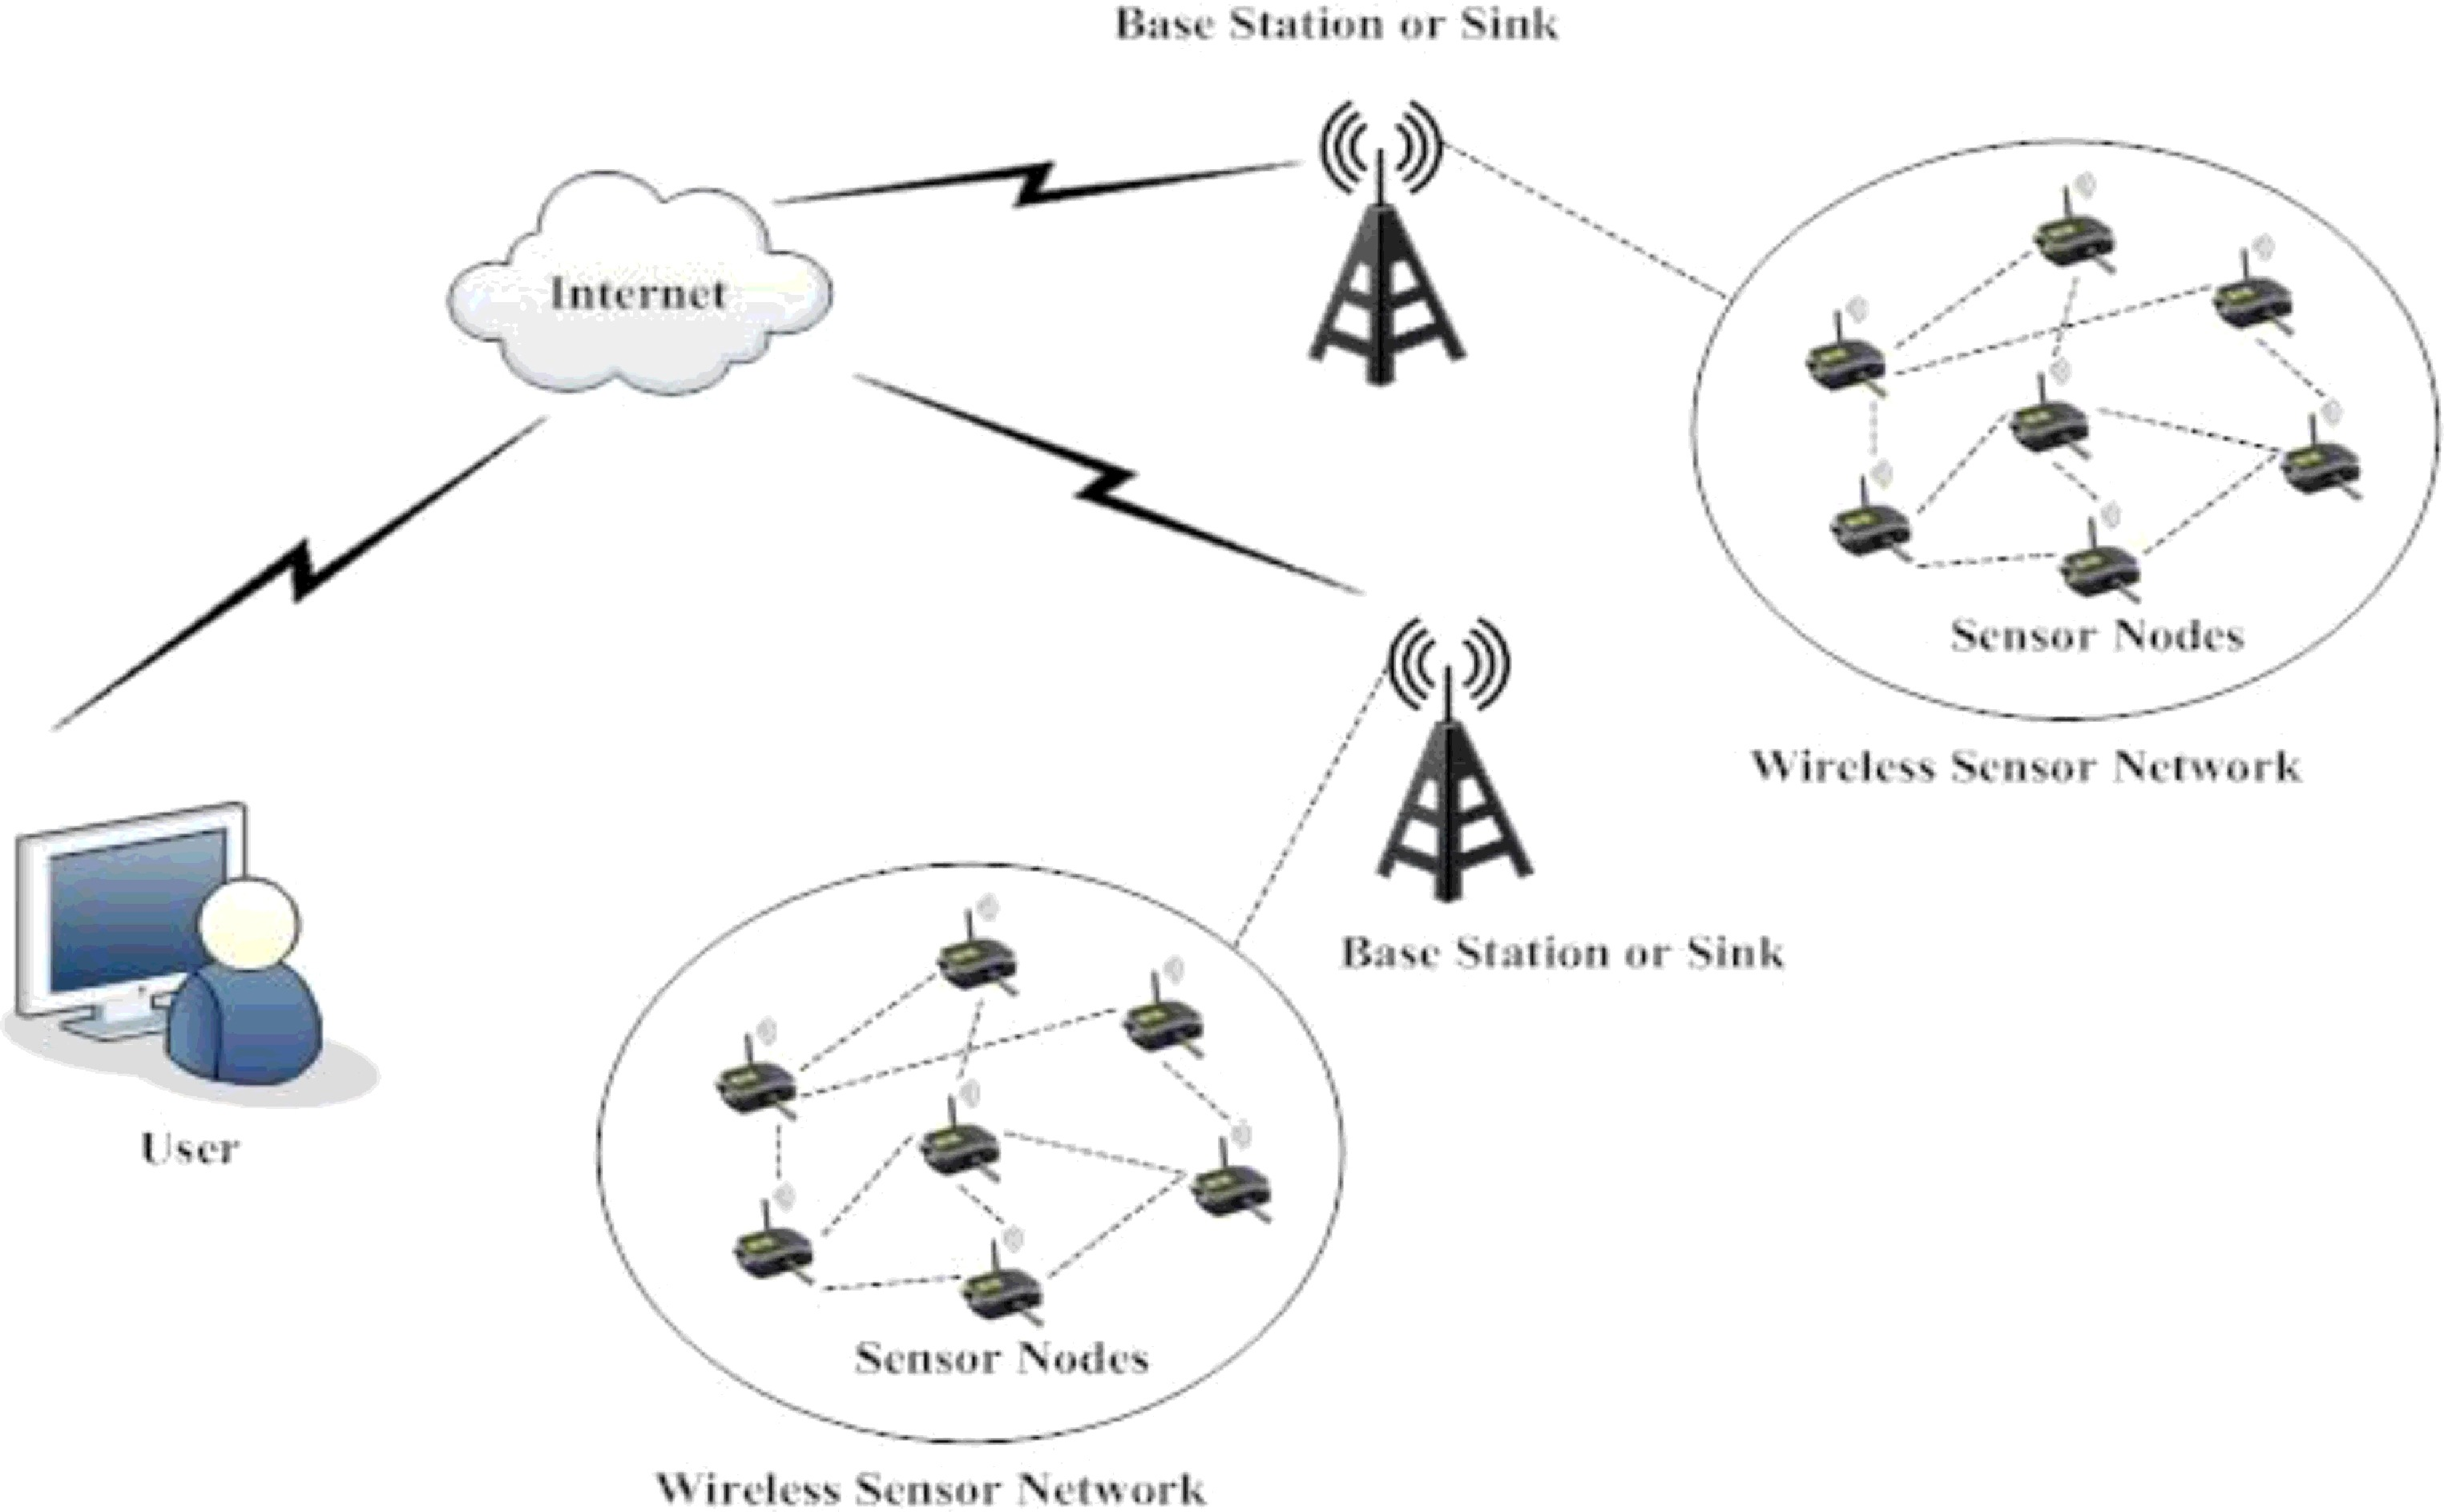
\includegraphics[width=\linewidth]{picture/wsn.jpg}
    
\end{frame}

\begin{frame}
    \frametitle{Ứng dụng}
    \begin{figure}
        \centering
        \subfigure[Nông nghiệp]{\fbox{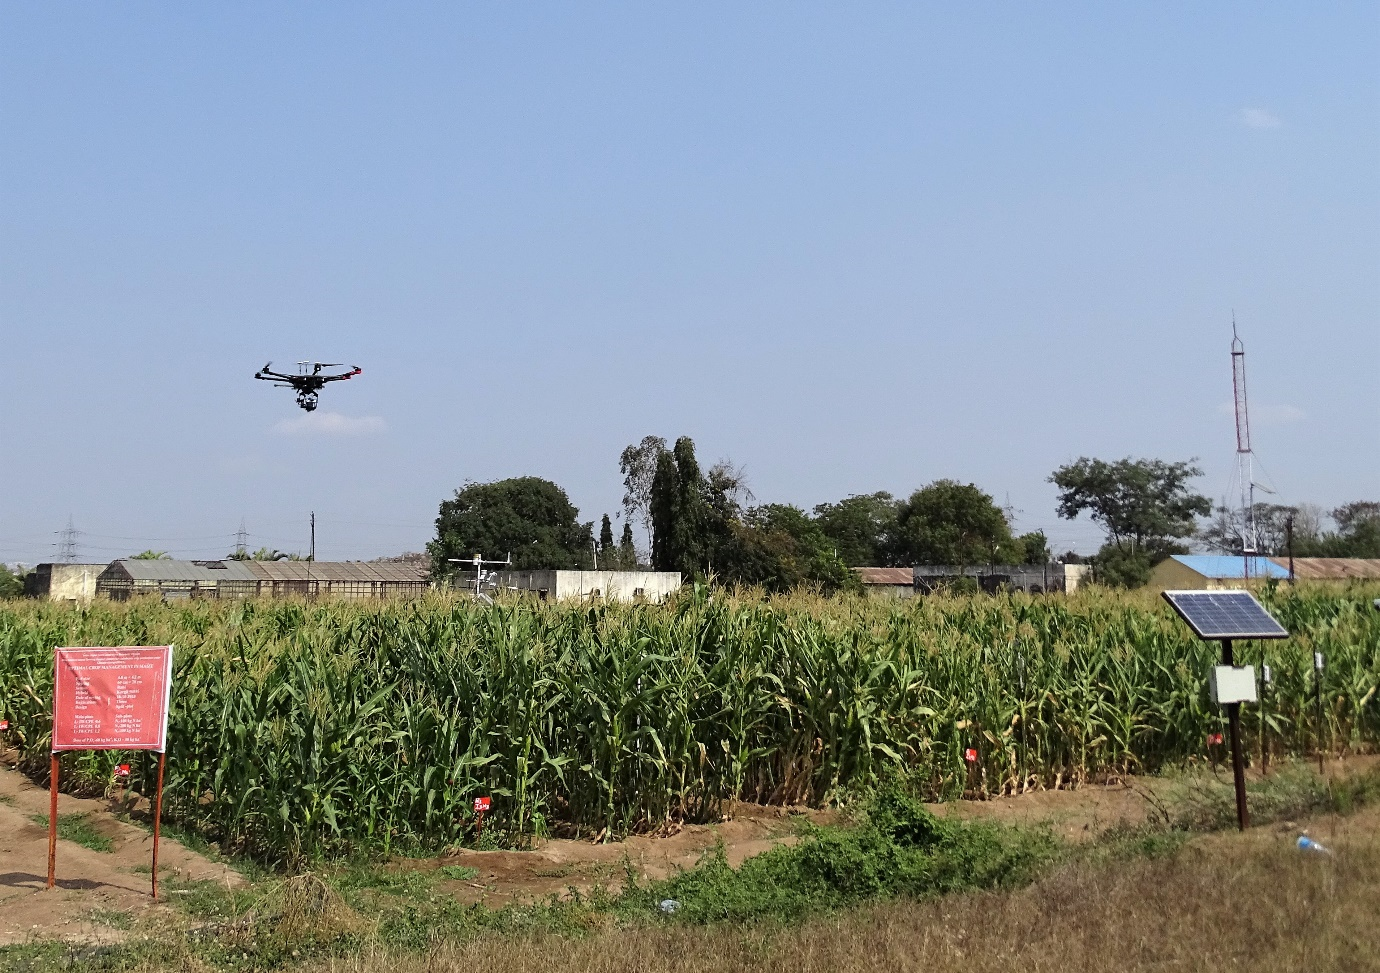
\includegraphics[width=0.45\linewidth, height=3cm]{picture/agri.png}}}
        \subfigure[Y tế]{\fbox{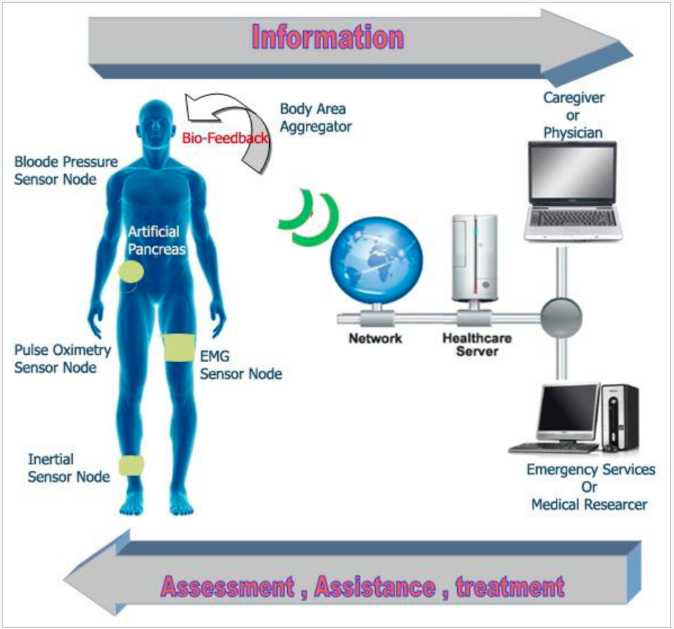
\includegraphics[width=0.45\linewidth, height=3cm]{picture/medical.png}}}
        \subfigure[Quân sự]{\fbox{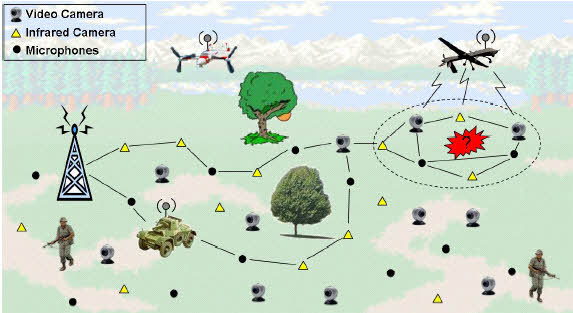
\includegraphics[width=0.45\linewidth, height=3cm]{picture/military.jpg}}}
        \subfigure[Nhà thông minh]{\fbox{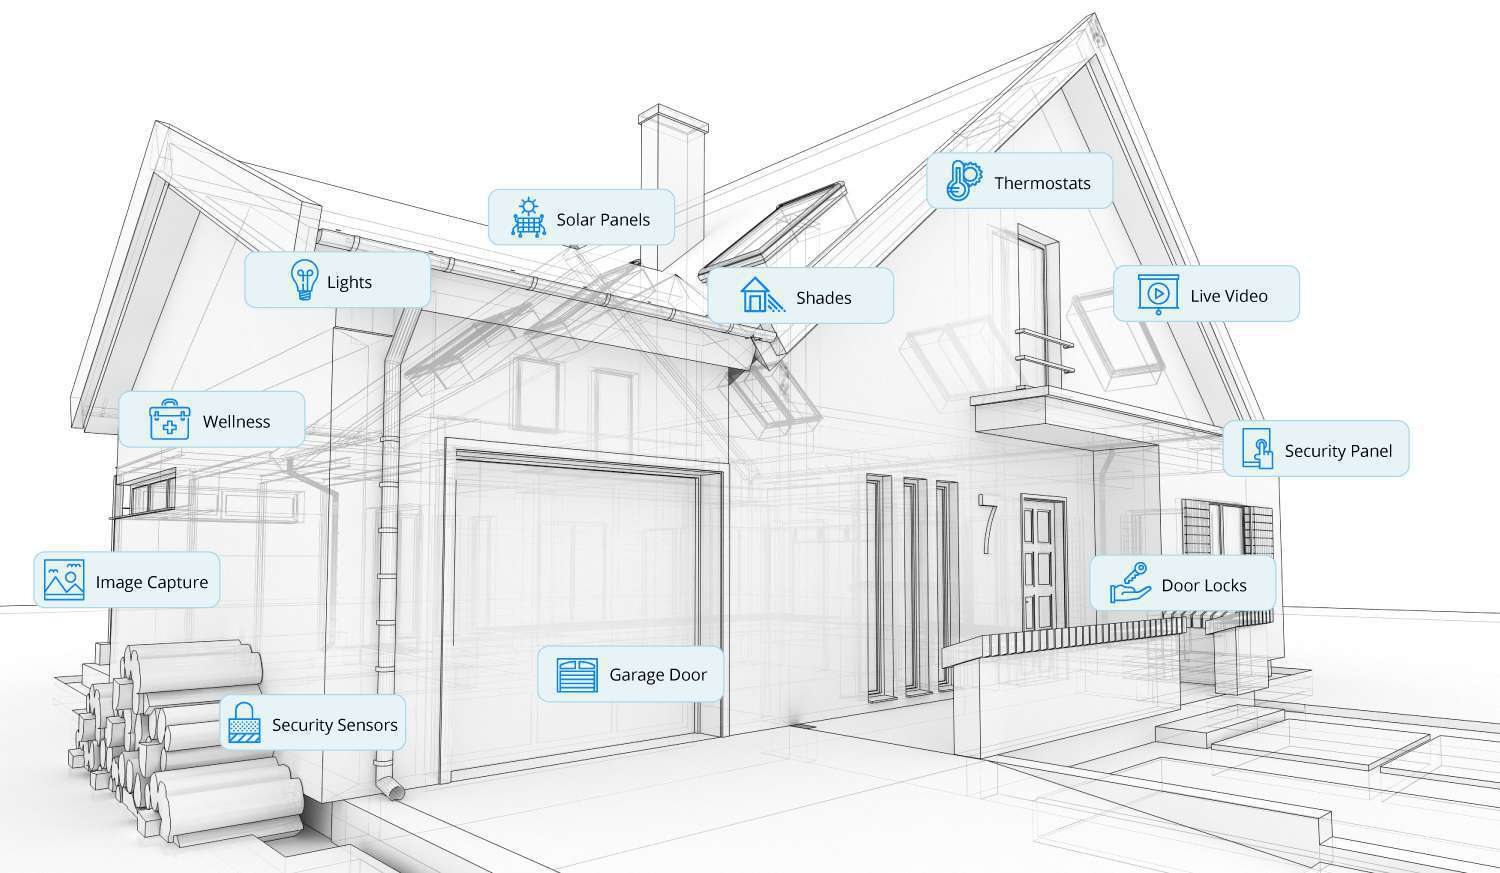
\includegraphics[width=0.45\linewidth, height=3cm]{picture/smart-home.jpg}}}
    \end{figure}
\end{frame}

\begin{frame}
    \frametitle{Thách thức}
    \begin{figure}
        \centering
        \subfigure[Bao phủ]{\fbox{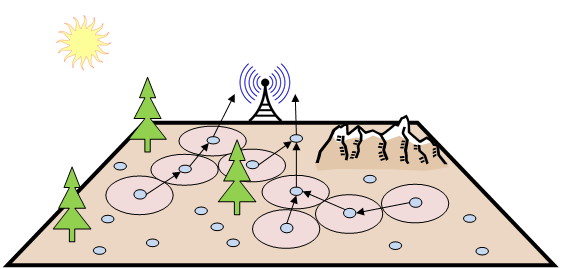
\includegraphics[width=0.45\linewidth, height=3cm]{picture/coverage.png}}}
        \subfigure[An ninh]{\fbox{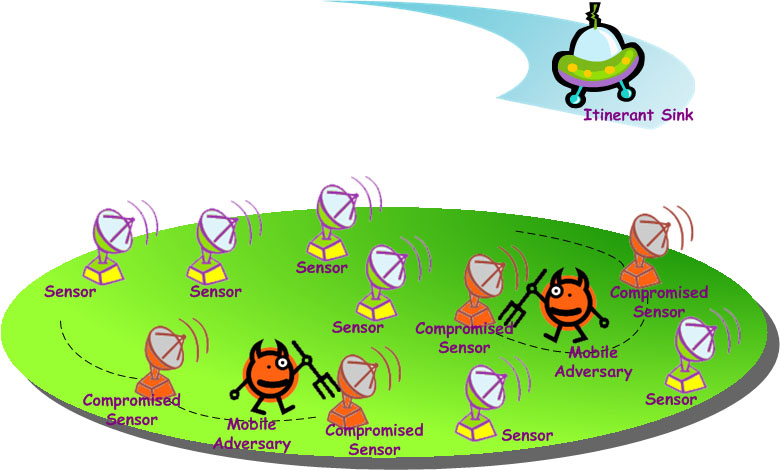
\includegraphics[width=0.45\linewidth, height=3cm]{picture/security.jpg}}}
        \subfigure[Định tuyến]{\fbox{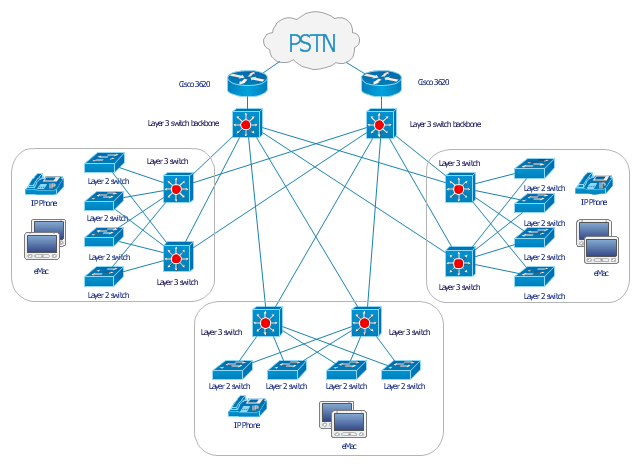
\includegraphics[width=0.45\linewidth, height=3cm]{picture/routing}}}
        \subfigure[Năng lượng]{\fbox{
\includegraphics[width=0.45\linewidth, height=3cm]{picture/charge.jpg}}}
    \end{figure}
    
\end{frame}

\begin{frame}
    \frametitle{Vấn đề tuổi thọ - hướng tiếp cận}
        
    \begin{figure}
        \subfigure[Phân cụm]{\fbox{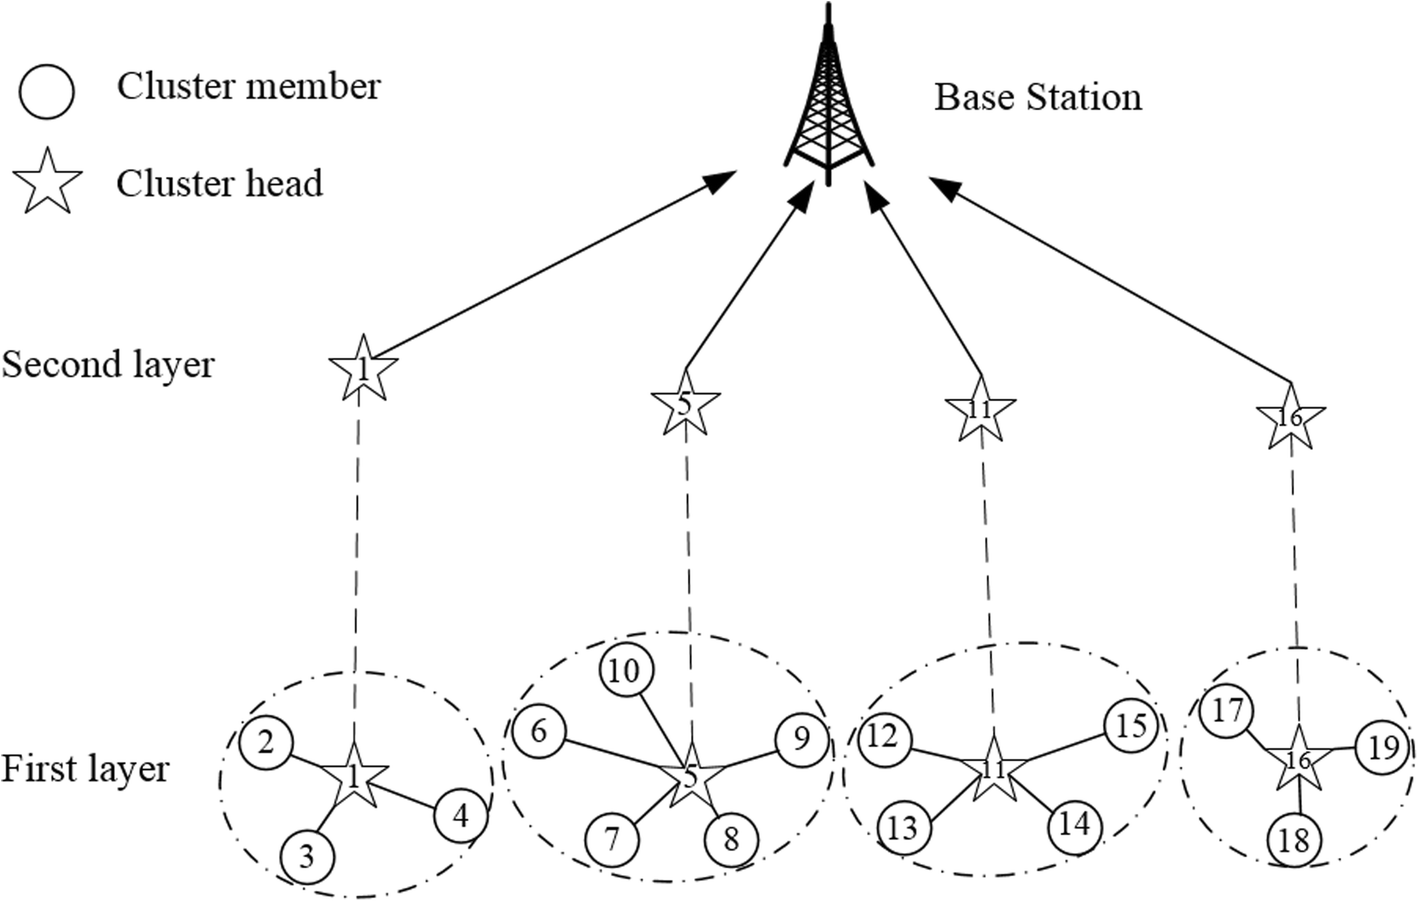
\includegraphics[width=0.5\linewidth, height=3cm]{picture/cluster.png}}}
        \subfigure[Đặt relay]{\fbox{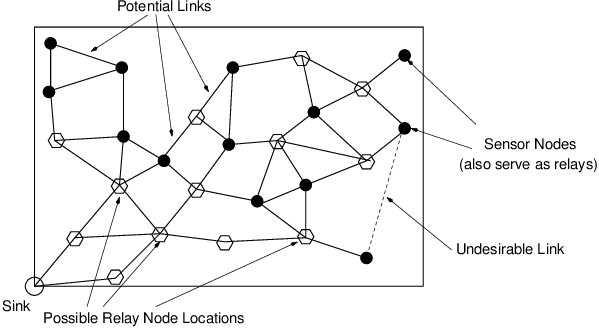
\includegraphics[width=0.5\linewidth, height=3cm]{picture/relay_placement.png}}}
    \end{figure}
\end{frame}

\begin{frame}
    \frametitle{Nghiên cứu liên quan}
    \begin{figure}
        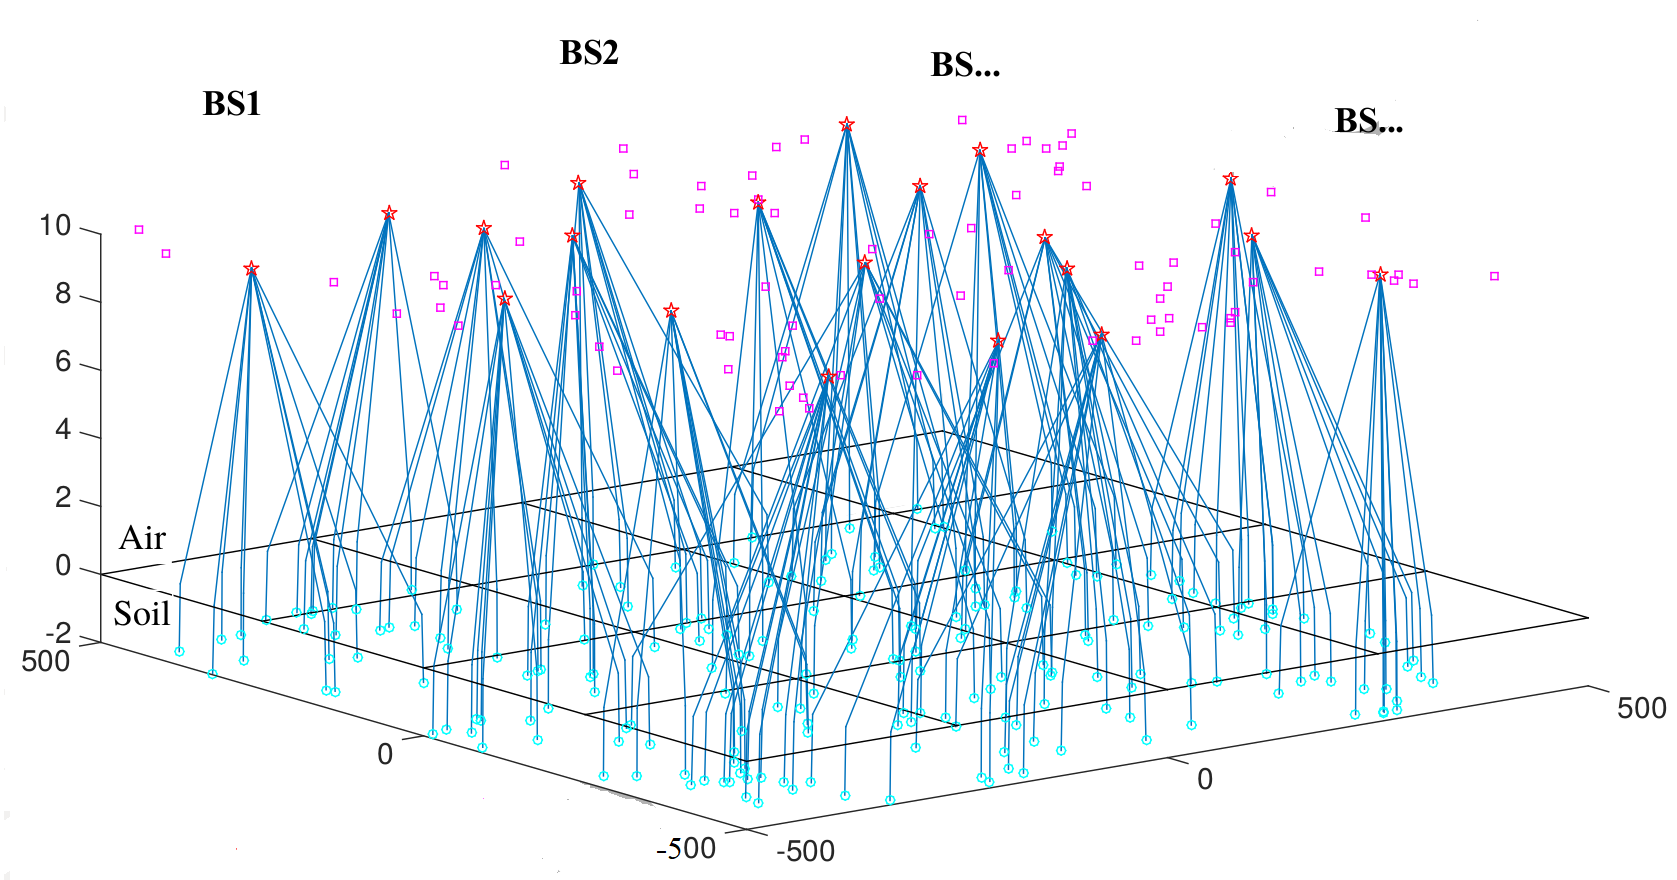
\includegraphics[width=\linewidth]{picture/yuan2017.png}
        \caption{Yuan et al. [2017]}
    \end{figure}
\end{frame}
\section{Bài toán tối ưu tuổi thọ trong mạng cảm biến không dây}

\begin{frame}
    \frametitle{Mô hình bài toán}
    \textbf{Đầu vào }
\begin{itemize}
    \item Không gian 3 chiều cần khảo sát với chiều dài và chiều rộng lần lượt là $W$ và $H$, chiều cao (sâu) vô hạn.
    \item $S = \{s_1, s_2,…, s_n\}$: tập các nút cảm biến được triển khai, mỗi nút cảm biến $s_i$ có các thuộc tính:
    \begin{itemize}
        \item[] $(xs_i, ys_i)$: tọa độ trên mặt $Oxy$
        \item[] $hs_i$: độ sâu so với mặt đất của cảm biến
        \item[] $r$: bán kính truyền thông 
        \item[] $l$: số bit mà nút cảm biến gửi tới trạm cơ sở
    \end{itemize}
    \item $F = \{f_1, f_2,…, f_m\}$: tập các vị trí khả thi để triển khai các nút chuyển tiếp, $f_i$ gồm các thuộc tính:
    \begin{itemize}
        \item[] $(xr_i, yr_i)$: tọa độ trên mặt $Oxy$
        \item[] $hr_i$: độ cao so với mặt đất của cảm biến
        \item[] $R$: bán kính truyền thông 
    \end{itemize}
\end{itemize}
\end{frame}

\begin{frame}
    \frametitle{Mô hình bài toán}
    \begin{itemize}
        \item $D = \{d_{11}, d_{12},…, d_{nm}\}$: ma trận khoảng cách 
    \begin{itemize}
        \item[] $d_{ij}$: khoảng cách từ sensor $s_i$ đến relay $f_j$
    \end{itemize}
    \item $C = \{c_{11}, c_{12},…, c_{nm}\}$: ma trận kết nối
    \begin{equation} 
        c_{ij} = \begin{cases}
            1 & \textrm{nếu $d_{ij} \leq r_i + R_j$}\\
            0 & \textrm{nếu ngược lại}
        \end{cases}
        \label{eqn:simple_one} 
    \end{equation}     
    \begin{itemize}
        \item[] Ý nghĩa: sensor $s_i$ có thể kết nối với relay $f_j$ nếu khoảng cách giữa hai nút không vượt quá tổng bán kính truyền thông của chúng
    \end{itemize}
    \item Năng lượng tiêu hao khi truyền $l$ bits dữ liệu từ sensor $s_i$ đến relay triển khai tại $f_j$
    \begin{equation}
        Et_{ij} = l * (E_{TX} + e_{fs} * d_{ij}^2)
        \label{sensor_consumption}
    \end{equation}
    \end{itemize}
\end{frame}

\begin{frame}
    \frametitle{Mô hình bài toán}
    \begin{itemize}
        \item Năng lượng tiêu hao của relay triển khai tại $f_j$ nhận dữ liệu từ $x_j$ sensors, tổng hợp và gửi tới trạm cơ sở
    \begin{equation}
        Er_j = l * (x_j * E_{RX} + x_j * E_{DA} + e_{mp} * d_{jtoBS}^4)
        \label{relay_consumption}
    \end{equation}
    \item $E_{max}$: năng lượng tiêu thụ tối đa mà một nút trong mạng có thể đạt đến
    \end{itemize}
\end{frame}

\begin{frame}
    \frametitle{Mô hình bài toán}
\textbf{Đầu ra }
\begin{itemize}
    \item $z = (z_1, z_2,…, z_m)$: vector quyết định
    \begin{equation}
        z_j = \begin{cases}
            1 & \textrm{nếu có relay triển khai tại $f_j$}\\
            0 & \textrm{nếu ngược lại}
        \end{cases}
    \end{equation}
    \item $A = \{a_{11}, a_{12},…, a_{nm}\}$: ma trận quyết định
    \begin{equation}
        a_{ij} = \begin{cases}
            1 & \textrm{nếu $s_i$ kết nối tới $f_j$}\\
            0 & \textrm{nếu ngược lại}
        \end{cases}
    \end{equation}
\end{itemize}

\end{frame}

\begin{frame}
    \frametitle{Mô hình bài toán}
\textbf{Ràng buộc }

\begin{equation}
    \sum_{j = 0}^m a_{ij} = 1 ~\forall i = 0, 1, \ldots, n: \textrm{mỗi sensor chỉ kết nối tới 1 relay}
\end{equation}
\begin{equation}
    z_j = a_{1j} \wedge a_{2j} \wedge \ldots \wedge a_{nj} ~\forall j = 1, 2, \ldots, m
\end{equation}

\textbf{Hàm mục tiêu }

\begin{equation}
    \frac{\alpha}{m} * \sum_{j = 1}^m z_j + \frac{1 - \alpha}{E_{max}} * E_x \rightarrow min
    \label{obj_func}
\end{equation}

Trong đó:
\begin{itemize}
    \item $E_x$ là năng lượng tiêu  hao lớn nhất của một nút trong lời giải. 
    \item $0 \leq \alpha \leq 1$: trọng số đánh giá độ quan trọng của số nút chuyển tiếp được sử dụng.
\end{itemize}
    
\end{frame}

\begin{frame}
    \frametitle{Hướng tiếp cận}
    \begin{itemize}
        \item Vét cạn 
        \item Các giải thuật xấp xỉ
    \end{itemize}
\end{frame}
\section{Các giải thuật đề xuất giải bài toán tối ưu tuổi thọ mạng cảm biến không dây}
\begin{frame}[noframenumbering]
  \frametitle{Nội dung trình bày}
  \tableofcontents[currentsection]
\end{frame}

\begin{frame}
    \frametitle{Ý tưởng}
    Giải bài toán theo 2 pha:
    \begin{itemize}
        \item Chọn ra các vị trí đặt nút chuyển tiếp.
        \item Tạo kết nối giữa nút cảm biến và nút chuyển tiếp.
    \end{itemize}
\end{frame}

\subsection{Giải thuật di truyền}
\begin{frame}
    \frametitle{Giải thuật di truyền}
    \textbf{Mã hóa cá thể}
    \begin{itemize}
        \item Sử dụng mã hóa nhị phân 
        \item $k = (k_1, k_2,…, k_m)$
        \item[] \begin{equation*}
            k_j = \begin{cases}
                1 & \textrm{nếu có relay triển khai tại $f_j$}\\
                0 & \textrm{nếu ngược lại}
            \end{cases}
        \end{equation*}
    \end{itemize} 
    
    Ví dụ: một cá thể với 10 vị trí khả thi đặt relay

    \begin{figure}[h]
        \centering
        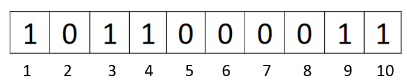
\includegraphics[width=7cm]{picture/indi_encoding.png}
        % \caption{Mã hóa cá thể }
    \end{figure}

    \textbf{Khởi tạo quần thể}

    Tạo ngẫu nhiên các dãy nhị phân độ dài m 
\end{frame}

\begin{frame}
    \frametitle{Giải thuật di truyền}
    
    \textbf{Lai ghép}

    Sử dụng lai ghép một điểm cắt, điểm cắt được chọn ngẫu nhiên
       
    \begin{figure}[h]
        \centering
        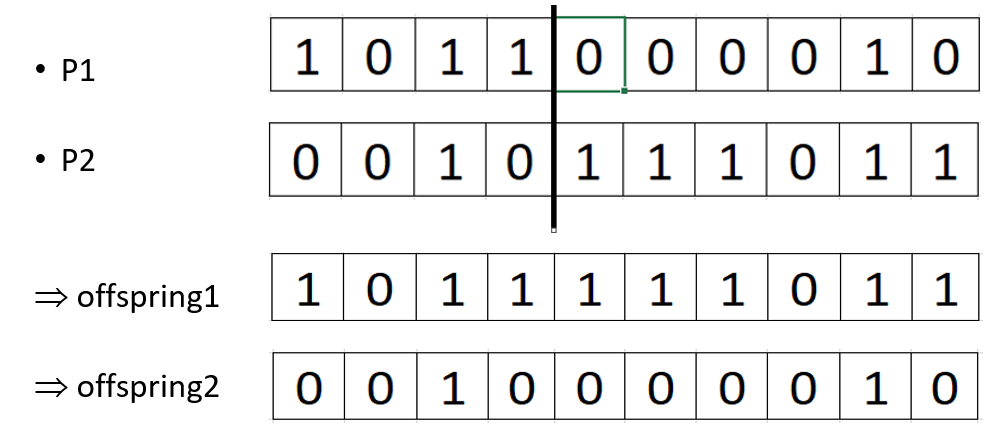
\includegraphics[width=8cm]{picture/crossover.png}
        % \caption{Mã hóa cá thể }
    \end{figure}

\end{frame}

\begin{frame}
    \frametitle{Giải thuật di truyền}
    
    \textbf{Đột biến}
    
    Chọn ngẫu nhiên một bit 0 và một bit 1 trong cá thể, hoán đổi vị trí chúng cho nhau 
       
    \begin{figure}[h]
        \centering
        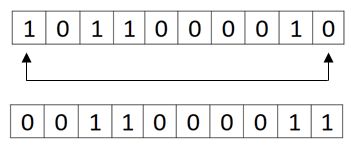
\includegraphics[width=5.5cm]{picture/mutation.png}
        % \caption{Mã hóa cá thể }
    \end{figure}
\end{frame}

\begin{frame}
    \frametitle{Giải thuật di truyền}
    
    \textbf{Tạo kết nối}
    
    Thuật toán heuristic lựa chọn kết nối: với từng nút cảm biến, lựa chọn nút chuyển tiếp sao cho phù hợp
\end{frame}

\begin{frame}
    \fontsize{10pt}{7pt}\selectfont
    \frametitle{Giải thuật di truyền}
       
    \begin{algorithm}[H]
        \SetKwData{Selid}{$sel\_id$}
        \SetKwData{Minmax}{min\_max}
        \SetKwData{Localmax}{local\_max}
        \SetKwData{lossone}{$loss_1$}
        \SetKwData{losstwo}{$loss_2$}
        \SetKwData{Sensors}{S}
        \SetKwData{Relays}{R}
        \SetKwData{Connect}{C}
        \SetKwData{TRUE}{True}
        \SetKwData{FALSE}{False}
        \SetKwData{esensor}{$Et$}
        \SetKwData{erelay}{$Er$}
        \SetKwData{varlthree}{$l_3$}
        \SetKwFunction{MAX}{Max}
        \SetKwFunction{ASSIGN}{Assign}
        \SetKwInOut{Input}{Đầu vào}
        \SetKwInOut{Output}{Đầu ra}
        % \Input{
        %     \\ \Sensors = $\{s_1, s_2, ..., s_n\}$ : tập các sensors 
        %     \\ \Relays = $\{r_1, r_2, ..., r_n\}$: tập các relays 
        %     \\ \Connect: ma trận kết nối 
        %     \\ \esensor, \erelay: năng  lượng tiêu hao của sensors và relays}
        % \Output{\\Các kết nối giữa sensors và relays}
            \SetAlgoLined
            \BlankLine
            \Begin{
                \For{$s_n \in \{s_1, s_2, ..., s_n\}$}{
                    $\Minmax \leftarrow$ INF \\
                    $\Selid \leftarrow 0$ \\
                    \For{$r_n \in \{r_1, r_2, ..., r_n\}$}{
                        $\lossone \leftarrow \esensor_{i, \Selid}$   \\
                        $\losstwo \leftarrow \erelay_j$ \\
                        $\Localmax \leftarrow \MAX(\lossone, \losstwo)$ \\
                        \If {\Minmax < \Localmax} {
                            $\Minmax \leftarrow \Localmax$ \\
                            $\Selid  \leftarrow j$
                        }
                    }
                    $\ASSIGN ~s_i$ to $r_{\Selid}$
                }
            }
            \caption{Connect ($S, R, C, Et, Er$)}      
    \end{algorithm}
\end{frame}

\begin{frame}
    \frametitle{Giải thuật di truyền}
    
    \textbf{Hàm thích nghi}

    Sử dụng hàm mục tiêu của mô hình là hàm thích nghi 

    \vspace{1cm}
    
    \textbf{Chọn lọc}

    \begin{itemize}
        \item Sắp xếp các cá thể theo độ thích nghi, chọn ra các cá thể có độ thích nghi tốt nhất.
        \item Trong trường hợp hai cá thể có độ thích nghi tương đương, sử dụng hàm mục tiêu phụ là tổng năng lượng tiêu hao trong mạng.
    \end{itemize}
   
\end{frame}

\subsection{Phương pháp tìm kiếm cục bộ}
\begin{frame}
    \frametitle{Phương pháp tìm kiếm cục bộ}

    \begin{figure}[h]
        \centering
        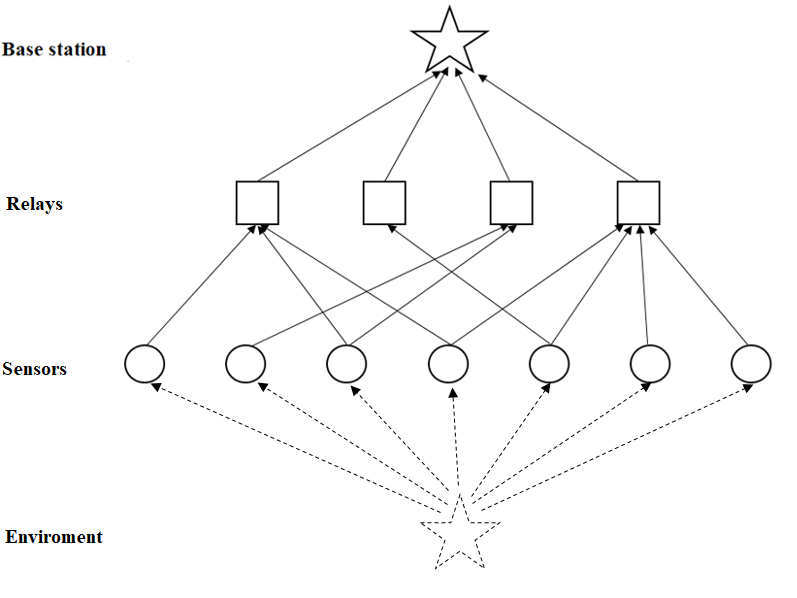
\includegraphics[width=0.9\linewidth]{picture/lite_flow.png}
        % \caption{Mã hóa cá thể }
    \end{figure}
\end{frame}

\begin{frame}
    \frametitle{Phương pháp tìm kiếm cục bộ}

    \textbf{Mã hóa lời giải}
    \begin{itemize}
        \item Vector $k = (k_1, k_2,…, k_m)$.
        \item Trong đó: 
        \begin{itemize}
            \item $k_j$ là số sensor mà relay $j$ kết nối, $1 \leq j \leq m$
            \item $k_j \leq q_j ~\forall 1 \leq j \leq m$ 
            \begin{equation*}
                q_j = \sum_{i = 1}^n c_{ij} ~\forall 1 \leq i \leq n
            \end{equation*}
            \begin{itemize}
                \item[] $q_j$ là số sensor tối đa relay $j$ có thể kết nối
                \item[] $C$ là ma trận kết nối đã nêu trên
            \end{itemize}
            \item Tổng số sensor mà các relay kết nối tới đúng bằng số sensor trong mạng.
            \begin{equation*}
                \sum_{j = 1}^m k_j = n
            \end{equation*}
        \end{itemize}
    \end{itemize}
\end{frame}


\begin{frame}
    \frametitle{Phương pháp tìm kiếm cục bộ}

    \textbf{Toán tử di chuyển}

    \begin{figure}[h!]
        \centering
        \subfigure[Swap]{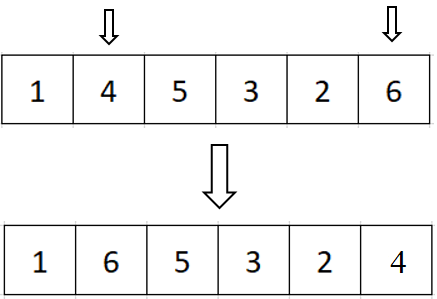
\includegraphics[width=0.35\linewidth]{picture/move1.png}}
        \hspace{1cm}
        \subfigure[Transfer]{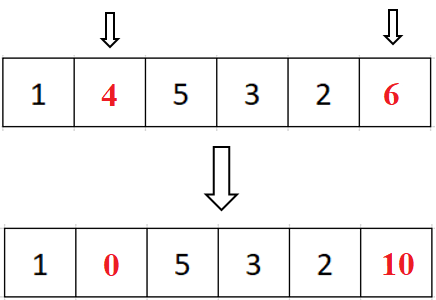
\includegraphics[width=0.35\linewidth]{picture/move2.png}}
        \subfigure[Up-down]{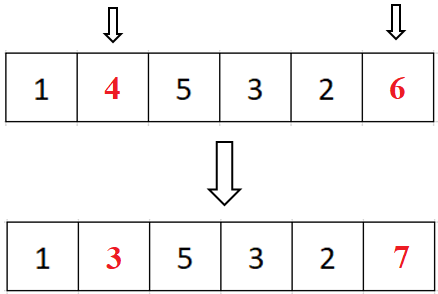
\includegraphics[width=0.35\linewidth]{picture/move3.png}}
    \end{figure}
\end{frame}

\begin{frame}
    \frametitle{Phương pháp tìm kiếm cục bộ}

    \textbf{Lượng giá lời giải}

    \begin{itemize}
        \item Sắp xếp tập các kết nối $E = \{e_1, e_2,…, e_k\}$ trong mạng theo thứ tự không giảm, tập các kết nối đã được sắp xếp $E’ = \{e'_1, e'_2,…, e'_k\}$.
        \item Tìm ra kết nối có chỉ  số nhỏ nhất $e'_i ~(1 \leq i \leq k)$ sao cho với các kết nối $e'_1, e'_2, …, e'_i$ ta giải được bài toán luồng cực đại trong mạng, việc tìm ra kết nối này dựa trên ý tưởng của tìm kiếm nhị phân.
    \end{itemize}
\end{frame}


% Ma gia thuat toan, tam thoi bo 
% \begin{frame}
%     \fontsize{9pt}{10pt}\selectfont
%     \frametitle{Phương pháp tìm kiếm cục bộ}

%     \begin{algorithm}[H]
%         \SetKwData{START}{start}
%         \SetKwData{MID}{mid}
%         \SetKwData{END}{end}
%         \SetKwData{Up}{up}
%         \SetKwData{Energy}{E'}
%         \SetKwData{ivar}{i}
%         \SetKwData{jvar}{j}
%         \SetKwData{TRUE}{True}
%         \SetKwData{FALSE}{False}
%         \SetKwData{varlone}{$l_1$}
%         \SetKwData{varltwo}{$l_2$}
%         \SetKwData{varlthree}{$l_3$}
%         \SetKwFunction{MaxFlow}{MaxFlow}
%         \SetKwFunction{FindConnect}{FindConnect}
%         \SetKwInOut{Input}{Đầu vào}
%         \SetKwInOut{Output}{Đầu ra}
%         % \Input{\\ \Energy : tập các kết nối đã được sắp xếp \\ \ivar và \jvar: chỉ số  bắt đầu và chỉ số kết thúc \\ Năng lượng tiêu hao của các kết nối trong mạng}
%         % \Output{\\Các kết nối được chọn}
%             \SetAlgoLined
%             \BlankLine
%             \Begin{
%                 $\START \leftarrow \ivar$\\
%                 $\END \leftarrow \jvar$\\
%                 $\MID \leftarrow \floor{(\START + \END)/2}$\\
%                 $\varlone \leftarrow \MaxFlow (e'_1, ..., e'_{start})$\\
%                 $\varltwo \leftarrow \MaxFlow (e'_1, ..., e'_{mid})$\\
%                 $\varlthree \leftarrow \MaxFlow (e'_1, ..., e'_{end})$\\
%                 \If{\varlone is \TRUE} {
%                 return $\{e'_1, ..., e'_{start}\}$
%                 }\If{\varlthree is \FALSE} {
%                 return \FALSE
%                 }
%                 \eIf{\varltwo is \FALSE} {
%                     return \FindConnect ($E', mid, end$)
%                 }{
%                     return \FindConnect ($E', start, mid$)
%                 }
%                 \DecMargin{1em}
%             }
%             \caption{FindConnect ($E', i, j$)}      
%     \end{algorithm}
% \end{frame}
\section{Kết quả thực nghiệm}
\begin{frame}[noframenumbering]
    \frametitle{Nội dung trình bày}
    \tableofcontents[currentsection]
  \end{frame}
\begin{frame}
    \frametitle{Dữ liệu thực nghiệm}
    Trích xuất từ một số khu vực thực tế

    \begin{table}[]
        \begin{tabularx}{\textwidth}{|l|l|X|}
            \hline
            \multicolumn{1}{|c|}{\textbf{Dữ liệu}} & \multicolumn{1}{c|}{\textbf{Khu vực thực tế}} & \multicolumn{1}{c|}{\textbf{Mô tả}}                                                                 \\ \hline
            T1 & Vũng Tàu                             & Thành phố nhiều tòa nhà với độ cao cân đối, có đồi núi, và một vùng biển nằm về một hướng  \\ \hline
            T2 & TP. HCM                           & Đồng bằng nhiều nhà cao tầng, ít sông                            \\ \hline
            T3 & Vĩnh Long                            & Ít nhà cửa, không đồi núi, kênh rạch nhiều đặc biệt có dòng sông lớn mekong                \\ \hline
            T4 & Lâm Đồng                             & Vùng đồi núi nhiều, ít nhà cửa, có núi cao, có sông xen kẽ                                \\ \hline
            T5 & Cao Nguyên                           & Vùng có nhiều đồi núi có độ cao tăng dần, ít nhà cửa, không sông hồ                        \\ \hline
            % dem7 & Đà Nẵng                              & Vùng ít nhà cửa, núi cao tiếp giáp vùng biển, vùng biển chủ yếu                            \\ \hline
            % dem8 & Hà Nội                               & Vùng nhiều nhà cao , có ao hồ                                                              \\ \hline
            % dem9 & Hạ Long                              & Vùng biển có nhiều đảo nhỏ độ cao khác nhau, không có nhà                                  \\ \hline
            % dem10 & Tây Bắc                             & Vùng thung lũng, thấp ở giữa và cao dần về hai bên                                         \\ \hline
        \end{tabularx}
        \caption{Mô tả địa hình thực nghiệm}
    \end{table}

\end{frame}

\begin{frame}
    \frametitle{Dữ liệu thực nghiệm}

    \begin{figure}
        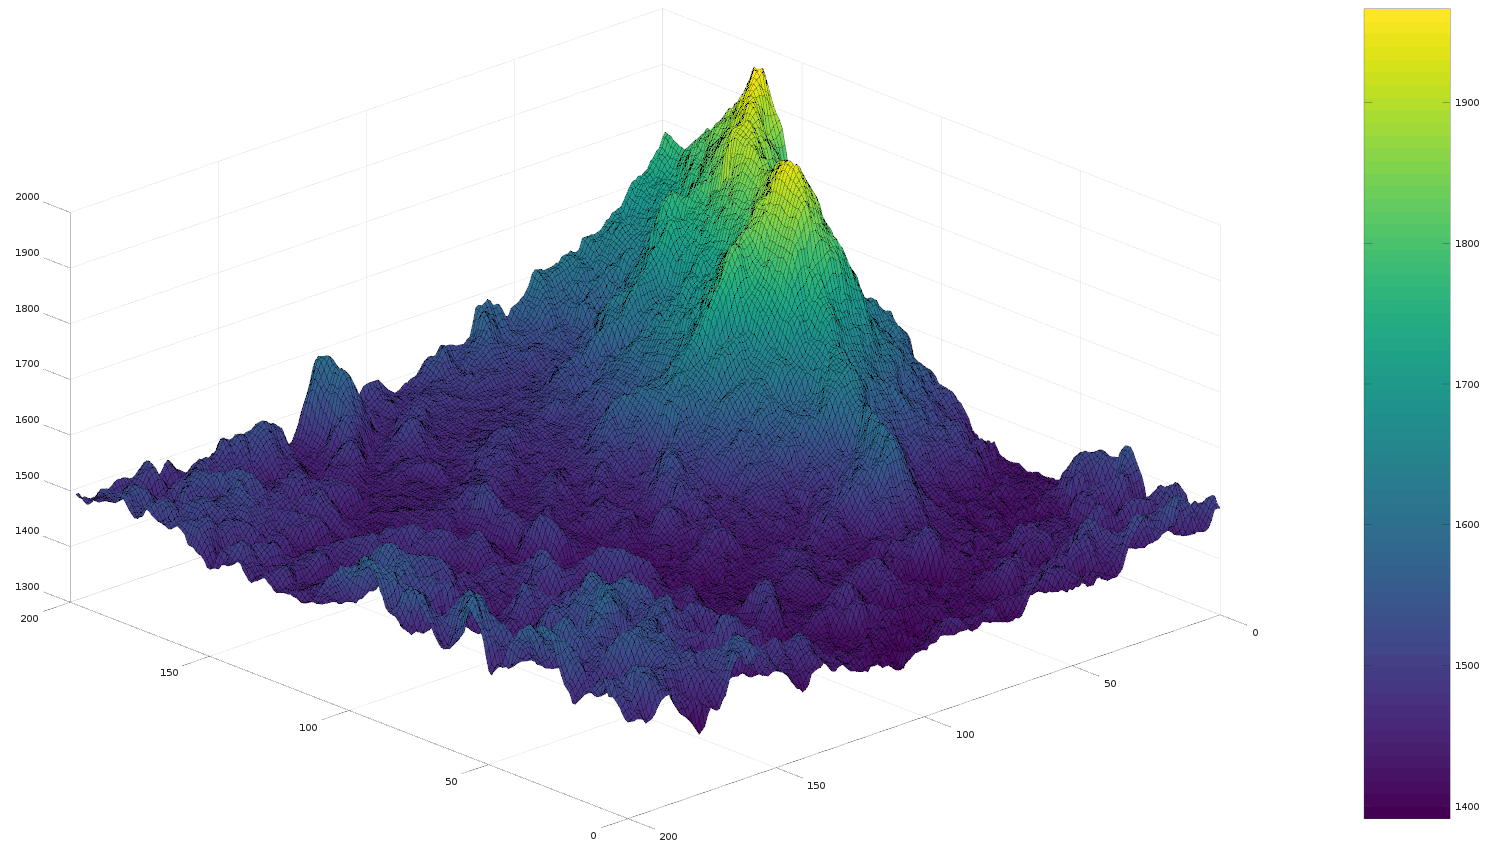
\includegraphics[width=\linewidth]{picture/Selection_038.png}
        \caption{Khu vực T4}
    \end{figure}
\end{frame}

\begin{frame}
    \frametitle{Tham số}
    Tham số chung của các bộ dữ liệu:
    \begin{itemize}
        \item Khu vực cảm  biến A là miền trong không gian 3 chiều với kích thước dài rộng là 200x200, chiều cao và sâu không hạn chế.
        \item Số sensor: 40  
        \item Sensor chôn sâu dưới mặt đất 10m
        \item Số vị trí khả thi đặt relay: 40 
        \item Vị trí đặt relay cao hơn mặt đất 1m
        \item $E_{TX}$ = 50*1e-9
        \item $E_{RX}$ = 50*1e-9
        \item $E_{DA}$ = 10*1e-12
        \item $e_{fs}$ = 10*1e-12
        \item $e_{mp}$ = 0.0013 * 1e-12
    \end{itemize}
\end{frame}

\begin{frame}
    \frametitle{Tham số}
    Tham số giải thuật di truyền:
    \begin{table}[H]
        \begin{tabularx}{\textwidth}{|X|X|}
            \hline
            \multicolumn{1}{|c|}{\textbf{Tham số}} & \multicolumn{1}{c|}{\textbf{Giá trị}}                    \\ \hline
            Số lần chạy 1 bộ dữ liệu  &  20                                                 \\ \hline
            Kích thước quần thể  & 100                                                      \\ \hline
            Số cá thể khởi tạo & 100                                                        \\ \hline
            Số thế hệ & 100                                                                 \\ \hline
            Số thế hệ dừng nếu không cải thiện kết quả & 30                                 \\ \hline
            Tỉ lệ lai ghép & 0.8                                                            \\ \hline
            Tỉ lệ đột biến   & 0.1                                                          \\ \hline
        \end{tabularx}
        \caption{Tham số cài thuật toán GAH}
    \end{table}
\end{frame}

\begin{frame}
    \frametitle{Kịch bản thử nghiệm}
    
    \begin{itemize}
        \item Cài đặt giải bài toán bằng mô hình quy hoạch nguyên nới lỏng.
        \item Chạy mỗi bộ dữ liệu 20 lần.
        \item $\alpha$ = 0.5
    \end{itemize}
\end{frame}

\begin{frame}
    \frametitle{Môi trường thực nghiệm}
    Thông số phần cứng:
    \begin{itemize}
        \item Bộ vi xử lý: Intel core i7-2640M 2.8GHz
        \item RAM: 4GB    
    \end{itemize}
\end{frame}

\begin{frame}
    \frametitle{So sánh kết quả}
    \begin{figure}[h!]
        \centering
        \subfigure{\fbox{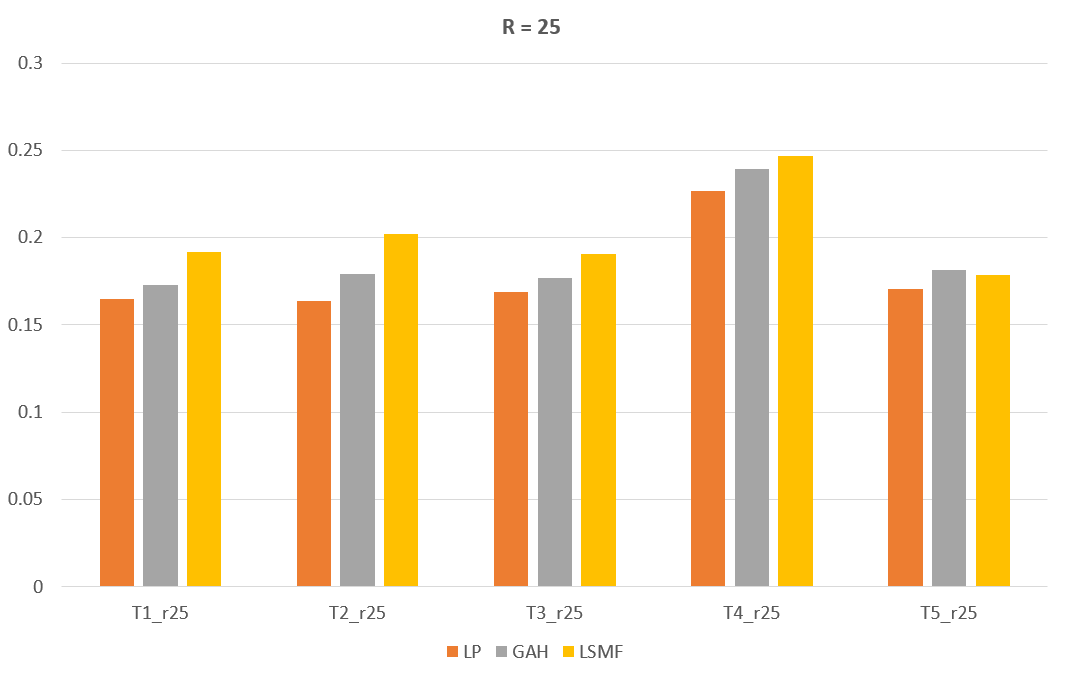
\includegraphics[width=0.4\linewidth, height=3.4cm]{picture/res_cp_25.png}}}
        \hspace{1cm}
        \subfigure{\fbox{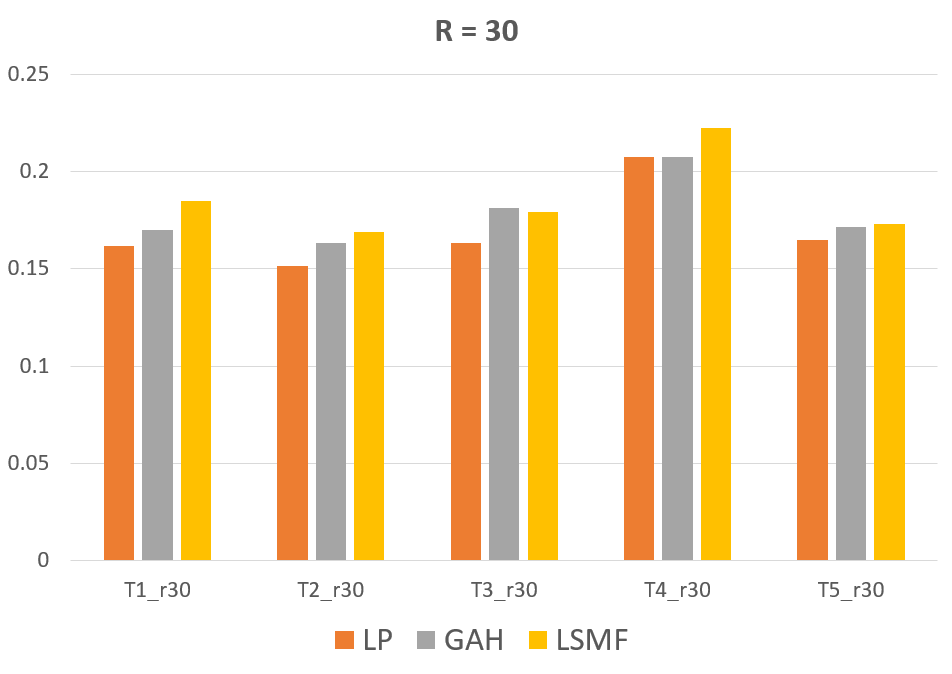
\includegraphics[width=0.4\linewidth]{picture/res_cp_30.png}}}
        \subfigure{\fbox{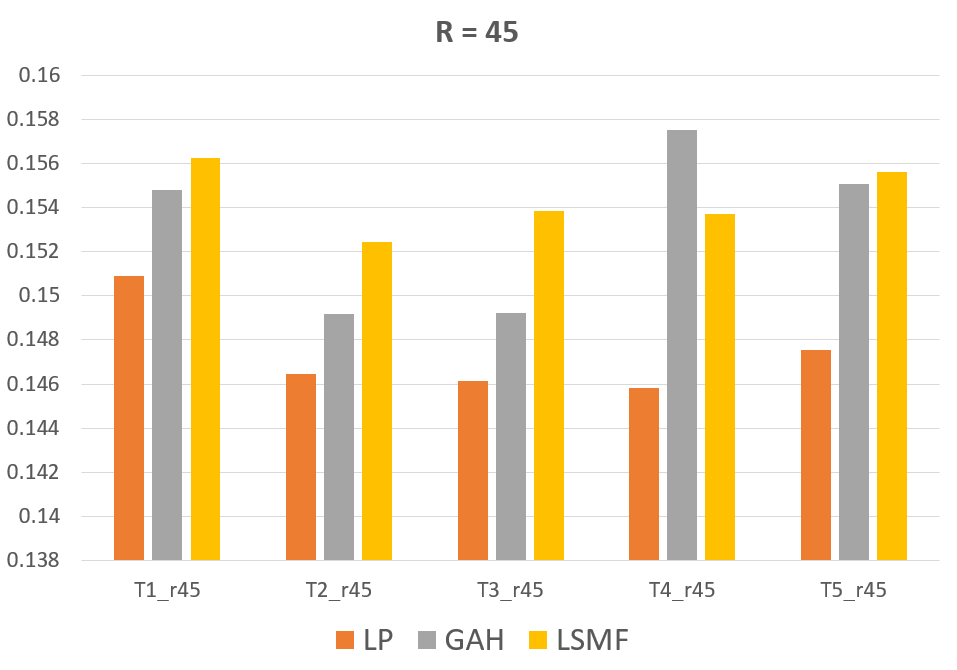
\includegraphics[width=0.4\linewidth]{picture/res_cp_45.png}}}
        \hspace{1cm}
        \subfigure{\fbox{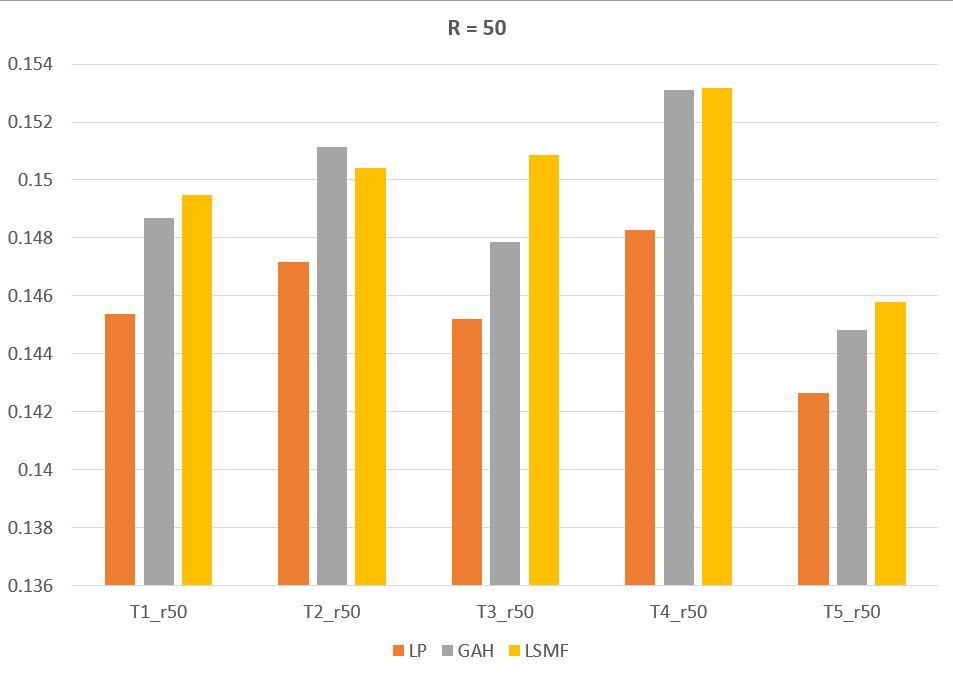
\includegraphics[width=0.4\linewidth]{picture/res_cp_50.png}}}
    \end{figure}
\end{frame}

\begin{frame}
    \frametitle{So sánh thời gian}
    \begin{figure}[h!]
        \centering
        \subfigure{\fbox{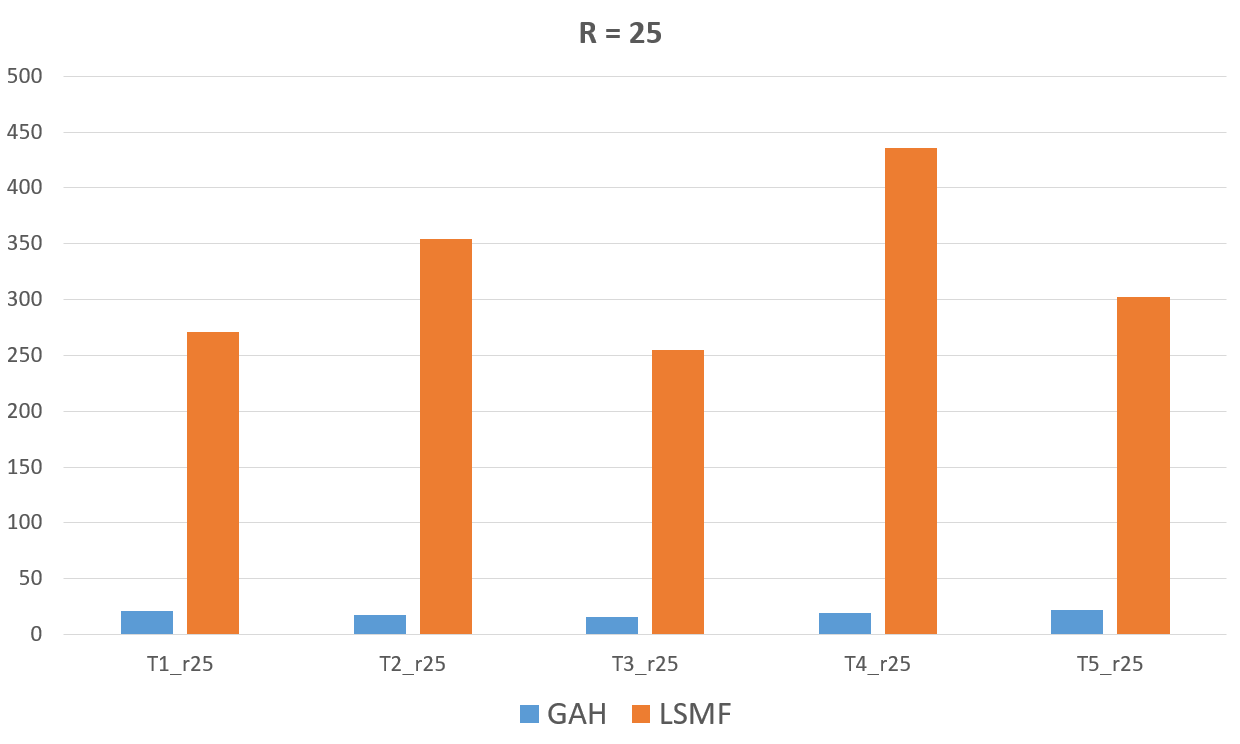
\includegraphics[width=0.4\linewidth]{picture/time_cp_25.png}}}
        \hspace{1cm}
        \subfigure{\fbox{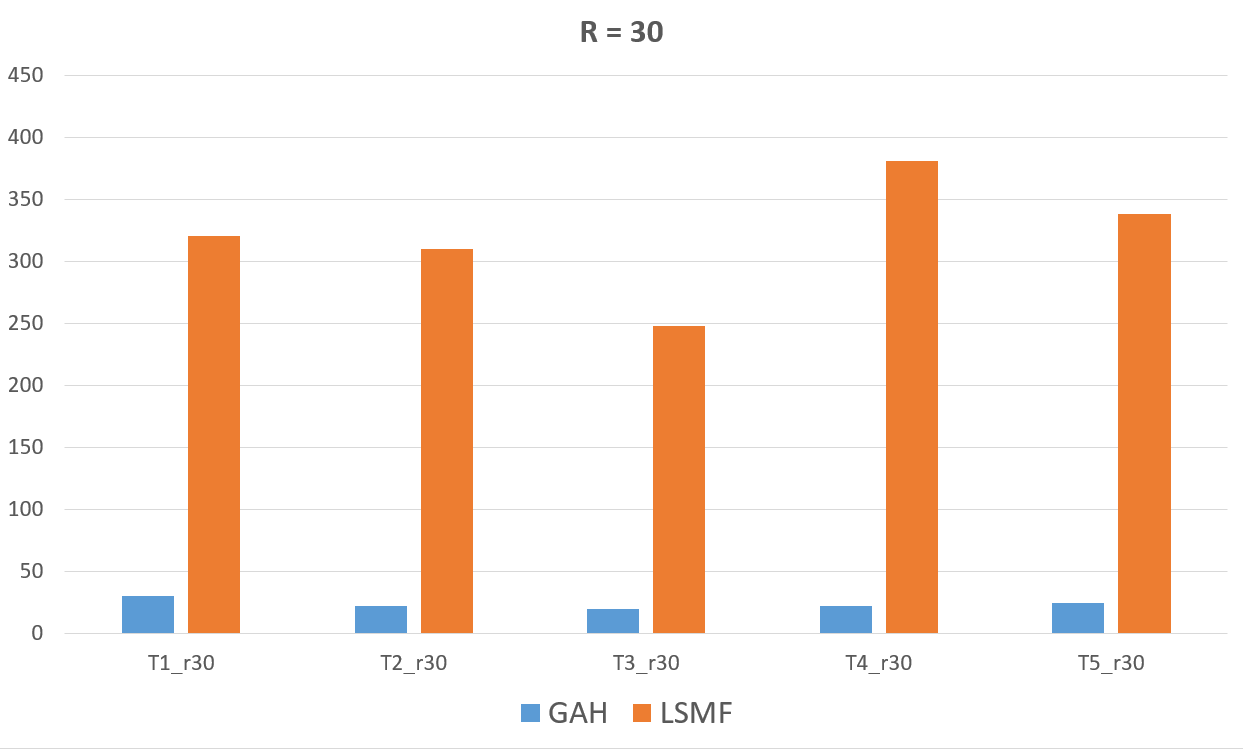
\includegraphics[width=0.4\linewidth]{picture/time_cp_30.png}}}
        \subfigure{\fbox{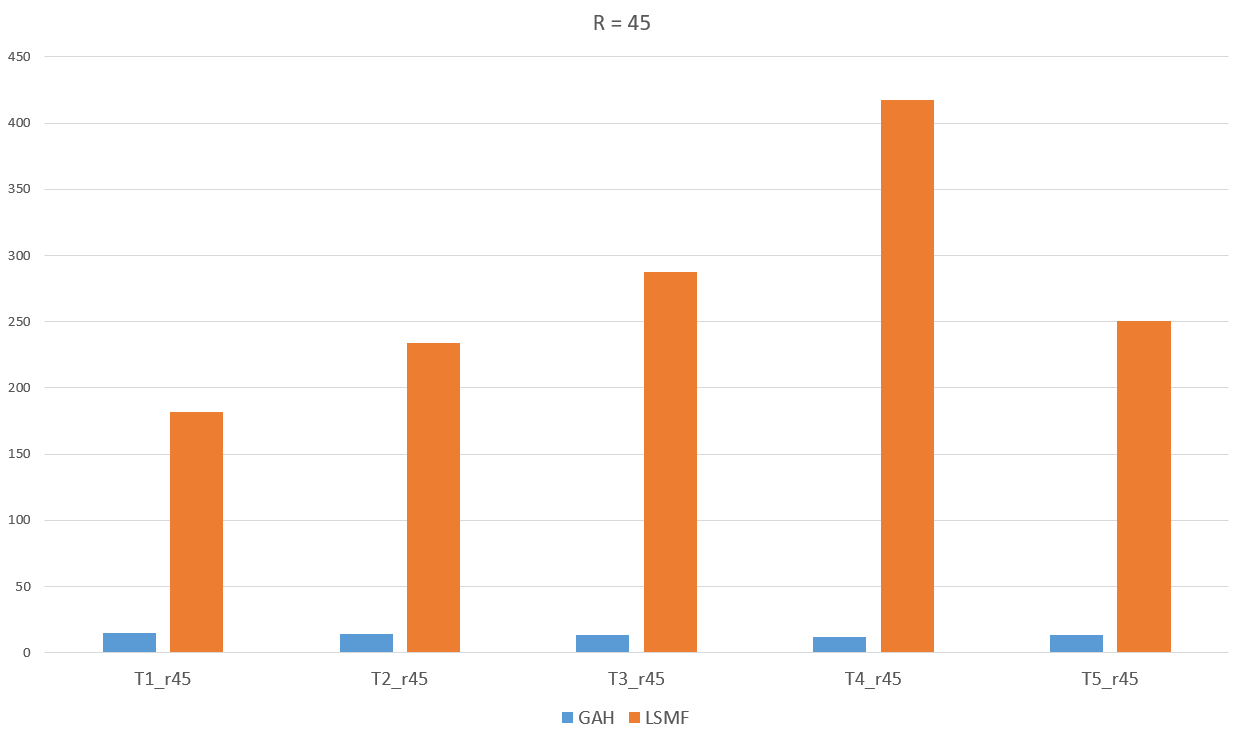
\includegraphics[width=0.4\linewidth]{picture/time_cp_45.png}}}
        \hspace{1cm}
        \subfigure{\fbox{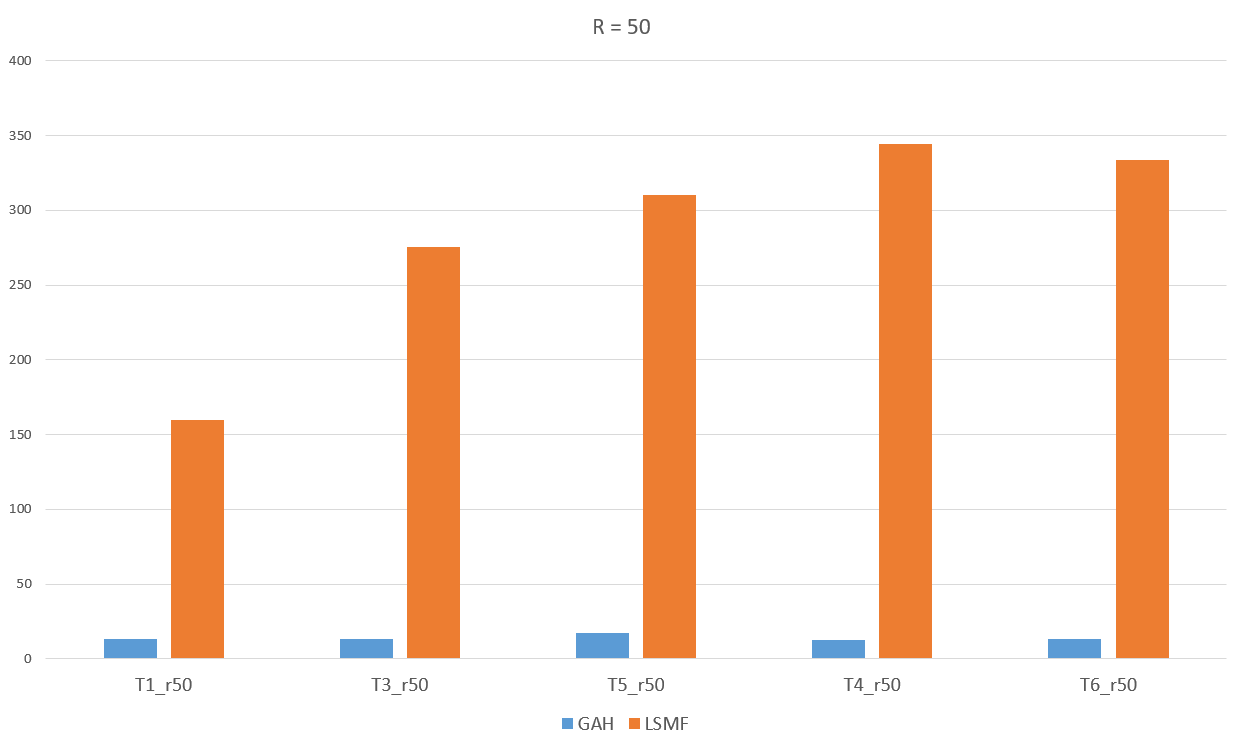
\includegraphics[width=0.4\linewidth]{picture/time_cp_50.png}}}
    \end{figure}
\end{frame}
\section{Kết luận}
\begin{frame}[noframenumbering]
    \frametitle{Nội dung trình bày}
    \tableofcontents[currentsection]
  \end{frame}

\begin{frame}
    \frametitle{Kết luận}

    \begin{itemize}
        \item Tìm hiểu bài toán tối ưu tuổi thọ mạng cảm biến không dây 
        \item Đề xuất giải thuật di truyền và phương pháp tìm kiếm cục bộ giải bài toán tối ưu thời gian sống mạng cảm biến không dây ngầm.
        \item Tiến hành cài đặt các giải thuật đề xuất.
        \item Thực nghiệm, so sánh, đánh giá kết quả.
    \end{itemize}
\end{frame}

\begin{frame}
    \Huge{\centerline{Thank you!}}
\end{frame}



\end{document} 